\documentclass[12pt]{article}

\usepackage{template/sbc-template}
\usepackage{graphicx,url}
\usepackage[utf8]{inputenc}
\usepackage[brazil]{babel}
% \usepackage[latin1]{inputenc}  

     
\sloppy

\title{Healthweb - sistema de diagnóstico especialista online}

\author{
Heitor Rodrigues Savegnago & 11077415 & heitor.rodrigues\inst{1}\\
Leopoldo Kenji Sugata Naves & 11201722022 & sugata.kenji\inst{1}\\
Otavio Lourenço da Silva & 13201812292 & otavio.silva\inst{1}
}

\address{\footnotesize\texttt{@aluno.ufabc.edu.br}}

\begin{document} 

\maketitle

% \begin{abstract}
%   This meta-paper describes the style to be used in articles and short papers
%   for SBC conferences. For papers in English, you should add just an abstract
%   while for the papers in Portuguese, we also ask for an abstract in
%   Portuguese (``resumo''). In both cases, abstracts should not have more than
%   10 lines and must be in the first page of the paper.
% \end{abstract}
     
\begin{resumo} 
  Atualmente no contexto nacional somente cerca de 30\% da população conta com um plano de saúde particular \cite{brunobocchini2018}, e muitas vezes, cerca de 40\% dos casos, o paciente brasileiro prefere fazer um autodiagnóstico baseado em informações retiradas da internet, que pode ser danoso à sua saúde \cite{vanessathees2018}.
  No presente trabalho é proposto um sistema online para diagnósticos simples, através de um linguajar menos técnico, e sempre deixando claro que procurar um médico antes de se automedicar é altamente recomendado.
  As bases de dados mais encontradas online trabalham com organização top down, listando doenças e descrevendo seu sintomas, fazendo até que o paciente desenvolva os demais sintomas da doença de forma psicossomática \cite{contaifercavalcante2018}.
  O diferencial desta proposta é a utilização de uma abordagem bottom up, obtendo e cruzando dados, através de questões a respeito de hábitos e sintomas do paciente, utilizando como amparo sistema de auxílio à tomada de decisão.
\end{resumo}
\section{Introdução}

Com o crescimento de informação e dados presentes na internet, houve um efeito exponencial na quantidade de aplicações/sites direcionados para praticamente qualquer conteúdo.
Ainda que possa-se dizer que a boa parte destes são direcionados para diversão e interações sociais, existem movimentos com o objetivo de facilitar e tranquilizar a quantidade esmagadora de usuários. Dentre esses, estão aqueles que se propositam a atividades como: compras essenciais e de materiais supérfluos, compra de medicamentos e  diagnóstico médico, sendo este último o foco deste trabalho.

Diagnósticos feitos por pesquisas simples em buscadores disponíveis hoje, em sua grande parte, nos atenta para doenças extremamente sérias, como câncer, embora os sintomas apresentados pelo usuário não tenham sido tão preocupantes.
Isto, pode nos levar para um quadro tão preocupante quanto, que seria o auto-diagnóstico baseado nestes resultados críticos, e um desenvolvimento de uma doença psicossomática, onde o paciente tem total certeza de que contêm a enfermidade apontada.
O objetivo deste, é explorar a relação de sintomas e doenças, lançando mão de um estudo estatístico, baseado na frequência em que se relacionam, ainda, cruzando essas informações com o perfil do paciente, para que o diagnóstico seja o mais assertivo possível, e não alarmante sem necessidade... ainda que sempre lembraremos, um diagnóstico profissional é imprescindível.
\section{Metodologia}

\subsection{Componentes}

A metodologia escolhida para a aplicação consiste num modelo \emph{Model View Controller} (MVC), onde cada camada será responsável por uma função, sendo estas:
\begin{itemize}
    \item \emph{Views}: tudo que diz respeito a interação com usuário, ou o questionário de sintomas.
    \item \emph{Controllers}: serão responsáveis pela comunicação com os dados sobre doenças e pela aplicação de lógica sobre os sintomas apresentados pelo usuário, também como quem devolverá os possíveis passos para prevenção e tratamento para o diagnóstico, nunca deixando de reforçar a necessidade de buscar ajuda profissional.
    \item \emph{Models}: serão as entidades que representarão os dados usado pela aplicação, ou seja, as doenças, sintomas, tratamentos e talvez algum dado ainda não previsto. Ainda fará, através de classes repositórios, a persistência dos dados no banco e consultas ao mesmo.
\end{itemize}

Tais camadas sendo devidamente encapsulada e fazendo a comunicação com as outras de forma segura e sem interferir no contexto.

\subsubsection{Views}

Também definido como \emph{front}, ou a interface vista pelo usuário. Será estruturada como um quiz, que apresentará questões booleanas, de verdadeiro ou falso, a respeito dos sintomas do paciente.
As informações obtidas neste formulário serão enviadas para a camada \emph{Controllers}.

\subsubsection{Controllers}

Aqui ocorre a interação do banco com as informações fornecidas pelo usuário, ou seja, questões simples sobre os sintomas registrados no banco serão enviadas para o \emph{front}, em seguida, a resposta voltará para a \emph{controller}.

Baseado nisso, será realizado um mapeamento, excluindo doença que não incluem os sintomas indicados e incluindo as demais, até que o sistema aponte uma possível resposta, devolvendo para o usuário o diagnóstico, uma possível prevenção e alguma forma de tratamento.
Sempre lembrando que a avaliação de qual diagnóstico adotar será baseada num índice de incidência que está em desenvolvimento e avaliação para melhor aproveitamento, citado na subseção \ref{ssec:models}.

\subsubsection{Models}\label{ssec:models}

Consiste no banco de dados, relacionando doenças a seus sintomas e alguns possíveis tratamentos.
Pretendemos definir um valor de probabilidade para esse relacionamento, para que tenha o papel de índice de tomada de decisão para a probabilidade do usuário apresentar a doença em questão baseado neste número.
Ainda não temos plena certeza de como calcular este valor de incidência, porém algumas bibliografias apresentam dados relevantes\cite{AlbertEinstein, longo2011harrison}.

\subsection{Opções similares}

Temos como referência de aplicação o Guia de Doenças e Sintomas \cite{AlbertEinstein}, tanto como possível base de dados a ser compilados, quanto em como forma de levar o questionário ao usuário.

Apresentando informações completas, é uma excelente ferramenta para sua proposta.
Por outro lado, também ilustra o cenário que desejamos evitar, quando o usuário recebe uma lista assustadora de doenças relacionadas ao seus sintomas, tais como câncer ou insuficiência renal, quando estão ligadas ao caso por poucos sintomas.

\subsection{Avaliação e conjunto de dados}

Avaliação: A avaliação da aplicação seria feita de forma ideal recebendo respostas de um paciente e validando o diagnóstico com um médico capacitado. Embora seja possível mensurar a efetividade com casos de teste, se escolhem doenças e inserindo respostas relacionadas ao sintomas da mesma, não deixando de conferir casos excepsionais, ou  em outras palavras, casos em que o usuário possa estar com sintomas divergentes.
Podem haver testes com usuários voluntários e até opiniões médicas.

\subsection{Complementação}

Respondendo aos questionamentos deixados pelo professor, não utilizaremos sistemas de análise de linguagem natural, já que a entrada do usuário será booleana, como sim ou não.
Não encontramos nenhum módulo disponível para este sistema, mas com uma análise estatística é possível criar uma base com margem de acerto aceeitável.
\section{Avaliação}

Uma avaliação preliminar da interface de usuário, utilizando o protótipo de média fidelidade foi realizada com um conjunto de cerca de cinco usuários, entre 20 e 30 anos, todos demonstraram satisfação para com o sistema e curiosidade pela implementação final.

O teste com um usuário de 52 anos foi realizado na versão final, o feedback apontou a boa praticidade no sistema, objetividade na apresentação de resultados e simplicidade na interface.

Outros testes de funcionamento do sistema foram realizados, a respeito do tratamento de erros internos ao servidor e lidando com páginas não encontradas pelo sistema, sempre apresentando uma página amigável ao usuário.

Algumas capturas da interface final são apresentadas na figura \ref{fig:desktop:final}, apresentando uma pergunta do banco de dados em \ref{fig:desktop:disease_real} e resultados em \ref{fig:desktop:results_real}.

\begin{figure}[htbp]
	\centering
	\begin{subfigure}{0.49\linewidth}
		\centering
		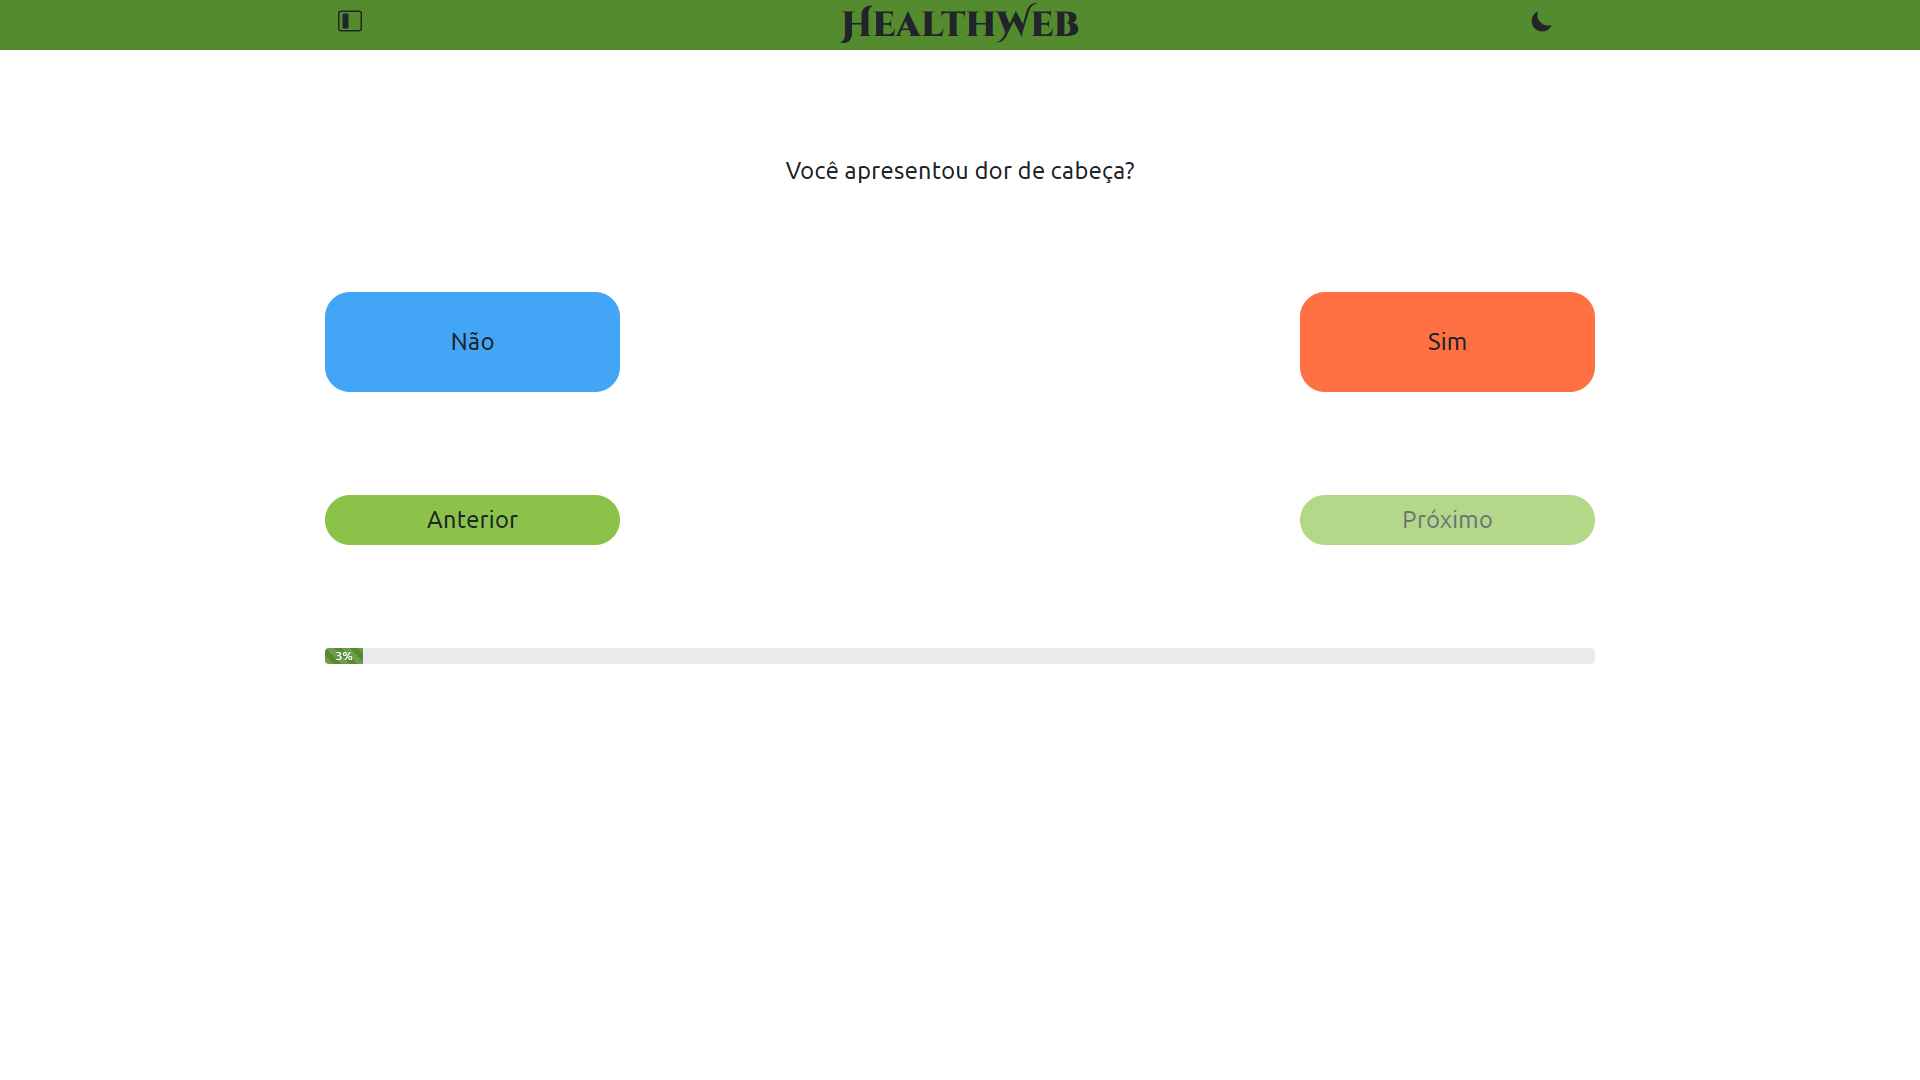
\includegraphics[width=\linewidth]{figure/disease_real.png}
		\caption{Tela de início.}
		\label{fig:desktop:disease_real}
	\end{subfigure}
	\hfill
	\begin{subfigure}{0.49\linewidth}
		\centering
		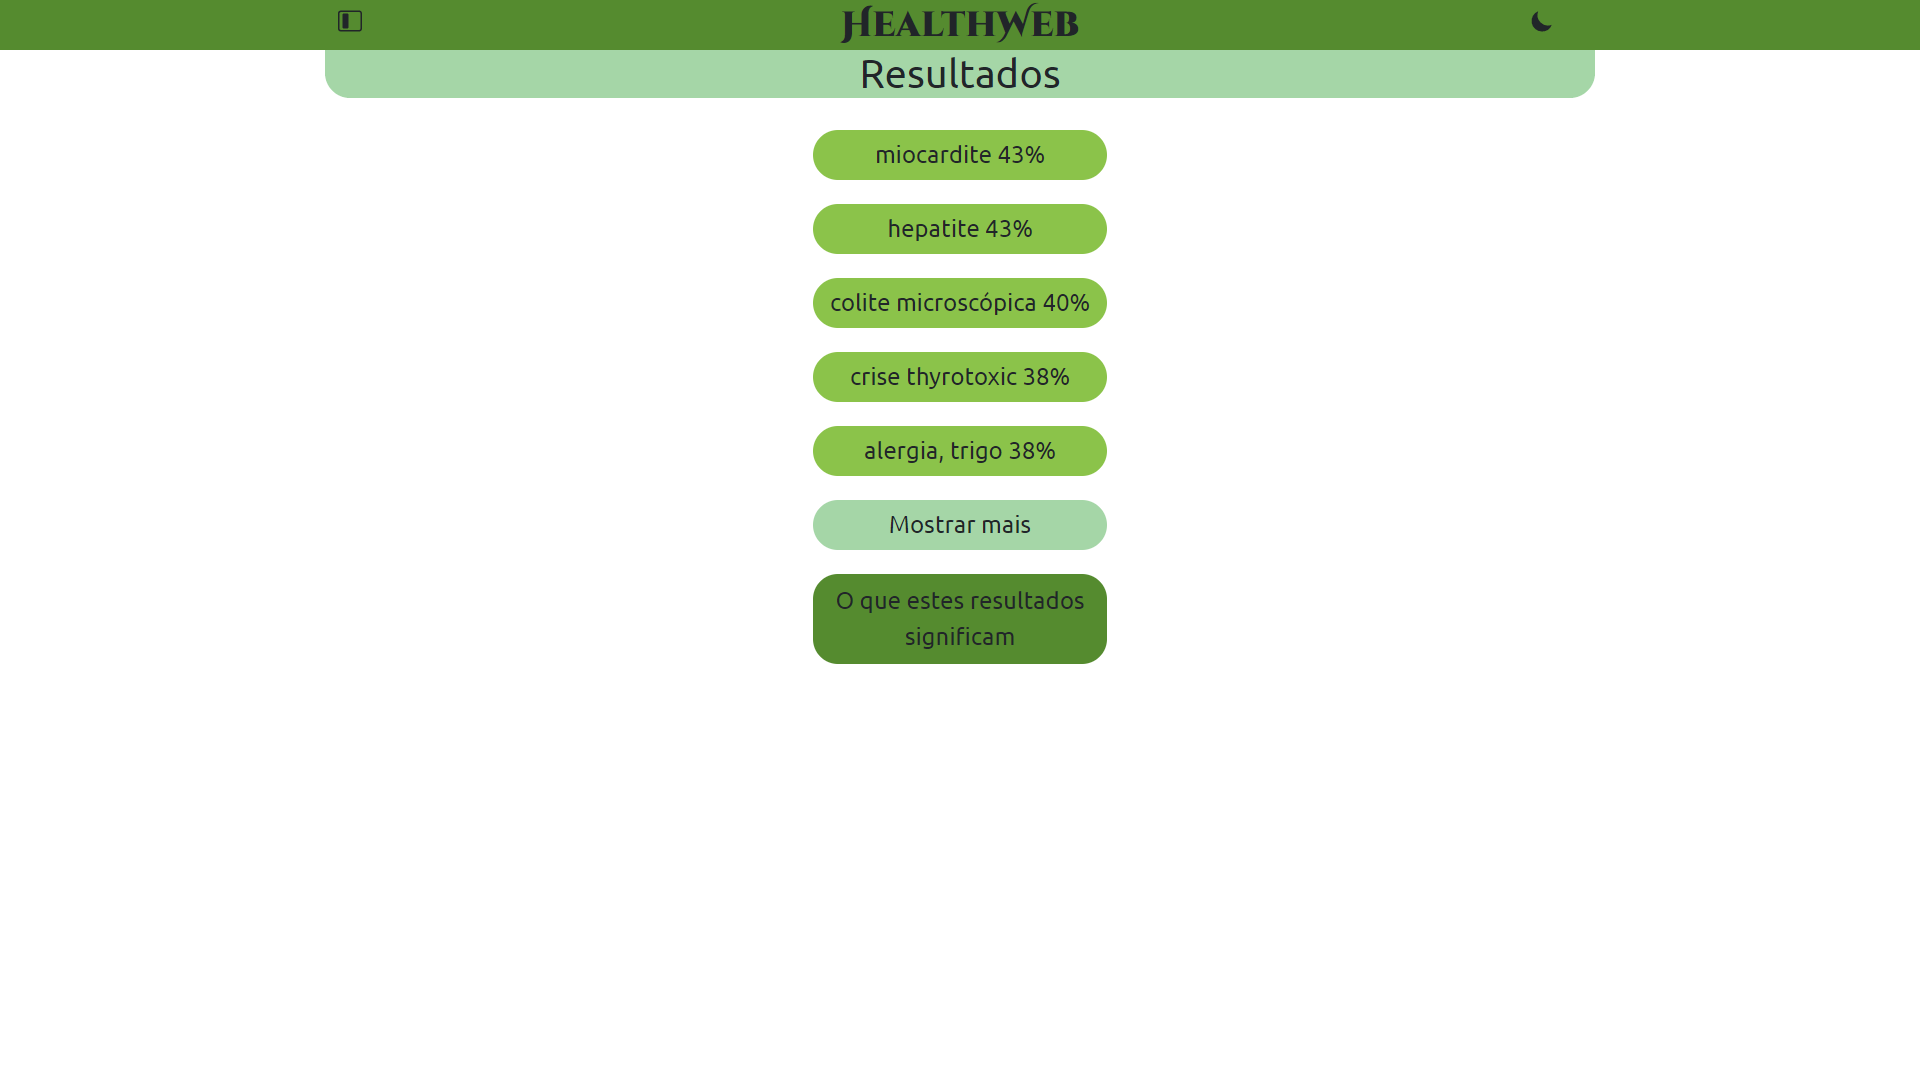
\includegraphics[width=\linewidth]{figure/results_real.png}
		\caption{Menu lateral recolhido na tela de início.}
		\label{fig:desktop:results_real}
	\end{subfigure}
	\caption{Tela de início e detalhe do menu lateral.}
	\label{fig:desktop:final}
\end{figure}




%Avaliação: A avaliação da aplicação seria feita de forma ideal recebendo respostas de um paciente e validando o diagnóstico com um médico capacitado. Embora seja possível mensurar a efetividade com casos de teste, se escolhem doenças e inserindo respostas relacionadas ao sintomas da mesma, não deixando de conferir casos excepcionais, ou  em outras palavras, casos em que o usuário possa estar com sintomas divergentes.
%Podem haver testes com usuários voluntários e até opiniões médicas.


\bibliographystyle{template/sbc}
\bibliography{sbc-template}

\end{document}
